%! TeX program = lualatex
%! TeX root = main.tex

\def\basedir{/home/theammir/labs/oop}
%! TeX program = lualatex
\documentclass[a4paper,14pt]{extarticle}
\usepackage[left=2.5cm,right=1.5cm,
		top=2cm,bottom=2cm,bindingoffset=0cm]{geometry}
\usepackage{fontspec}
\usepackage{fancyhdr}
\usepackage{fancyvrb}
\setmainfont{FreeSerif}
\setmonofont{FiraCode}
\usepackage[english,ukrainian]{babel}
\usepackage[position=bottom]{caption}

\usepackage{minted}
\setminted{style=arduino}
\setminted{mathescape}

\usepackage{caption}
\captionsetup[listing]{name=Файл}

\pagestyle{fancy}
\fancyhead{}
\fancyfoot[C]{}
\fancyfoot[R]{\thepage}
\setlength{\headheight}{17pt}
\renewcommand{\headrulewidth}{0pt}

\setcounter{secnumdepth}0

\newcommand{\shell}[2][build/temp.tex]{%
	\immediate\write18{#2 > #1}%
	\CatchFileDef{\out}{#1}{\endlinechar=13}%
}

\newcommand{\codefile}[2]{%
	\begin{center}
		\inputminted[tabsize=2, breaklines, fontsize=\small]{#1}{\basedir/\thelabid/#2}
		\captionof{listing}{\detokenize{#2}}
	\end{center}
}

\newcommand{\thetitlepage}[4]{
	\def\thelabno{#1}
	\def\thelabid{\thelabno}
	\def\thestudentno{#4}
	
	\begin{titlepage}
	\begin{center}
		\vspace{1cm}
		\textbf{Міністерство освіти і науки України\\
		Національний технічний університет України\\
		<<Київський політехнічний інститут імені Ігоря Сікорського>>\\
		Факультет інформатики та обчислювальної техніки\\
		Кафедра обчислювальної техніки\\}
		\vspace*{5cm}
		\textbf{Лабораторна робота №#1\\}
		\vspace{0.5cm}
		з дисціпліни\\
		<<Об'єктно-орієнтоване програмування>>
		\vspace*{7cm}
		
		\begin{tabular}{ll}
		\begin{minipage}[t]{0.54\linewidth}
			Виконав:\\
			студент групи #2\\
			#3\\
			номер у списку групи: \thestudentno\par
		\end{minipage}
		&
		\begin{minipage}[t]{0.3\linewidth}
			Перевірив:\\
			Порєв В.~М.
		\end{minipage}
		\end{tabular}

		\vfill
		Київ \the\year\\
	\end{center}
	\end{titlepage}
	\setcounter{page}2
}

\newcommand{\taskdesc}{\section*{Завдання}}

\newcommand{\taskspec}{\section{Варіант \thestudentno}}

\newcommand{\codetext}{\section{Текст програм}}

\newcommand{\tasktest}{\section{Результати тестування програми}}

\newcommand{\conclusion}{\section{Висновок}}

% vim: ts=2: sw=2


\usepackage{graphicx}

\begin{document}
\thetitlepage{2}{ІМ-42}{Туров Андрій Володимирович}{26}
\def\thelabid{lab2}

\taskspec%
Варіант Ж = 26:
\begin{enumerate}
	\item Статичний масив \texttt{*shapes[126]}.
	\item Слід --- суцільна лінія синього кольору.
	\item Увід прямокутника --- від кута до кута.
	\item Прямокутник --- блакитний, з чорним контуром.
	\item Увід еліпса --- від центру до кута прямокутника.
	\item Еліпс --- білий, з чорним контуром.
	\item В меню має позначатись поточний об'єкт, що вводиться.
\end{enumerate}
  

\codetext%
\codefile{cpp}{src/main.cpp}
\codefile{cpp}{src/canvas.h}
\codefile{cpp}{src/canvas.cpp}
\codefile{cpp}{src/editor.h}
\codefile{cpp}{src/editor.cpp}
\codefile{cpp}{src/shape.h}
\codefile{cpp}{src/shape.cpp}
\codefile{cmake}{CMakeLists.txt}

\section{Зображення}

\begin{figure}[h!]
  \center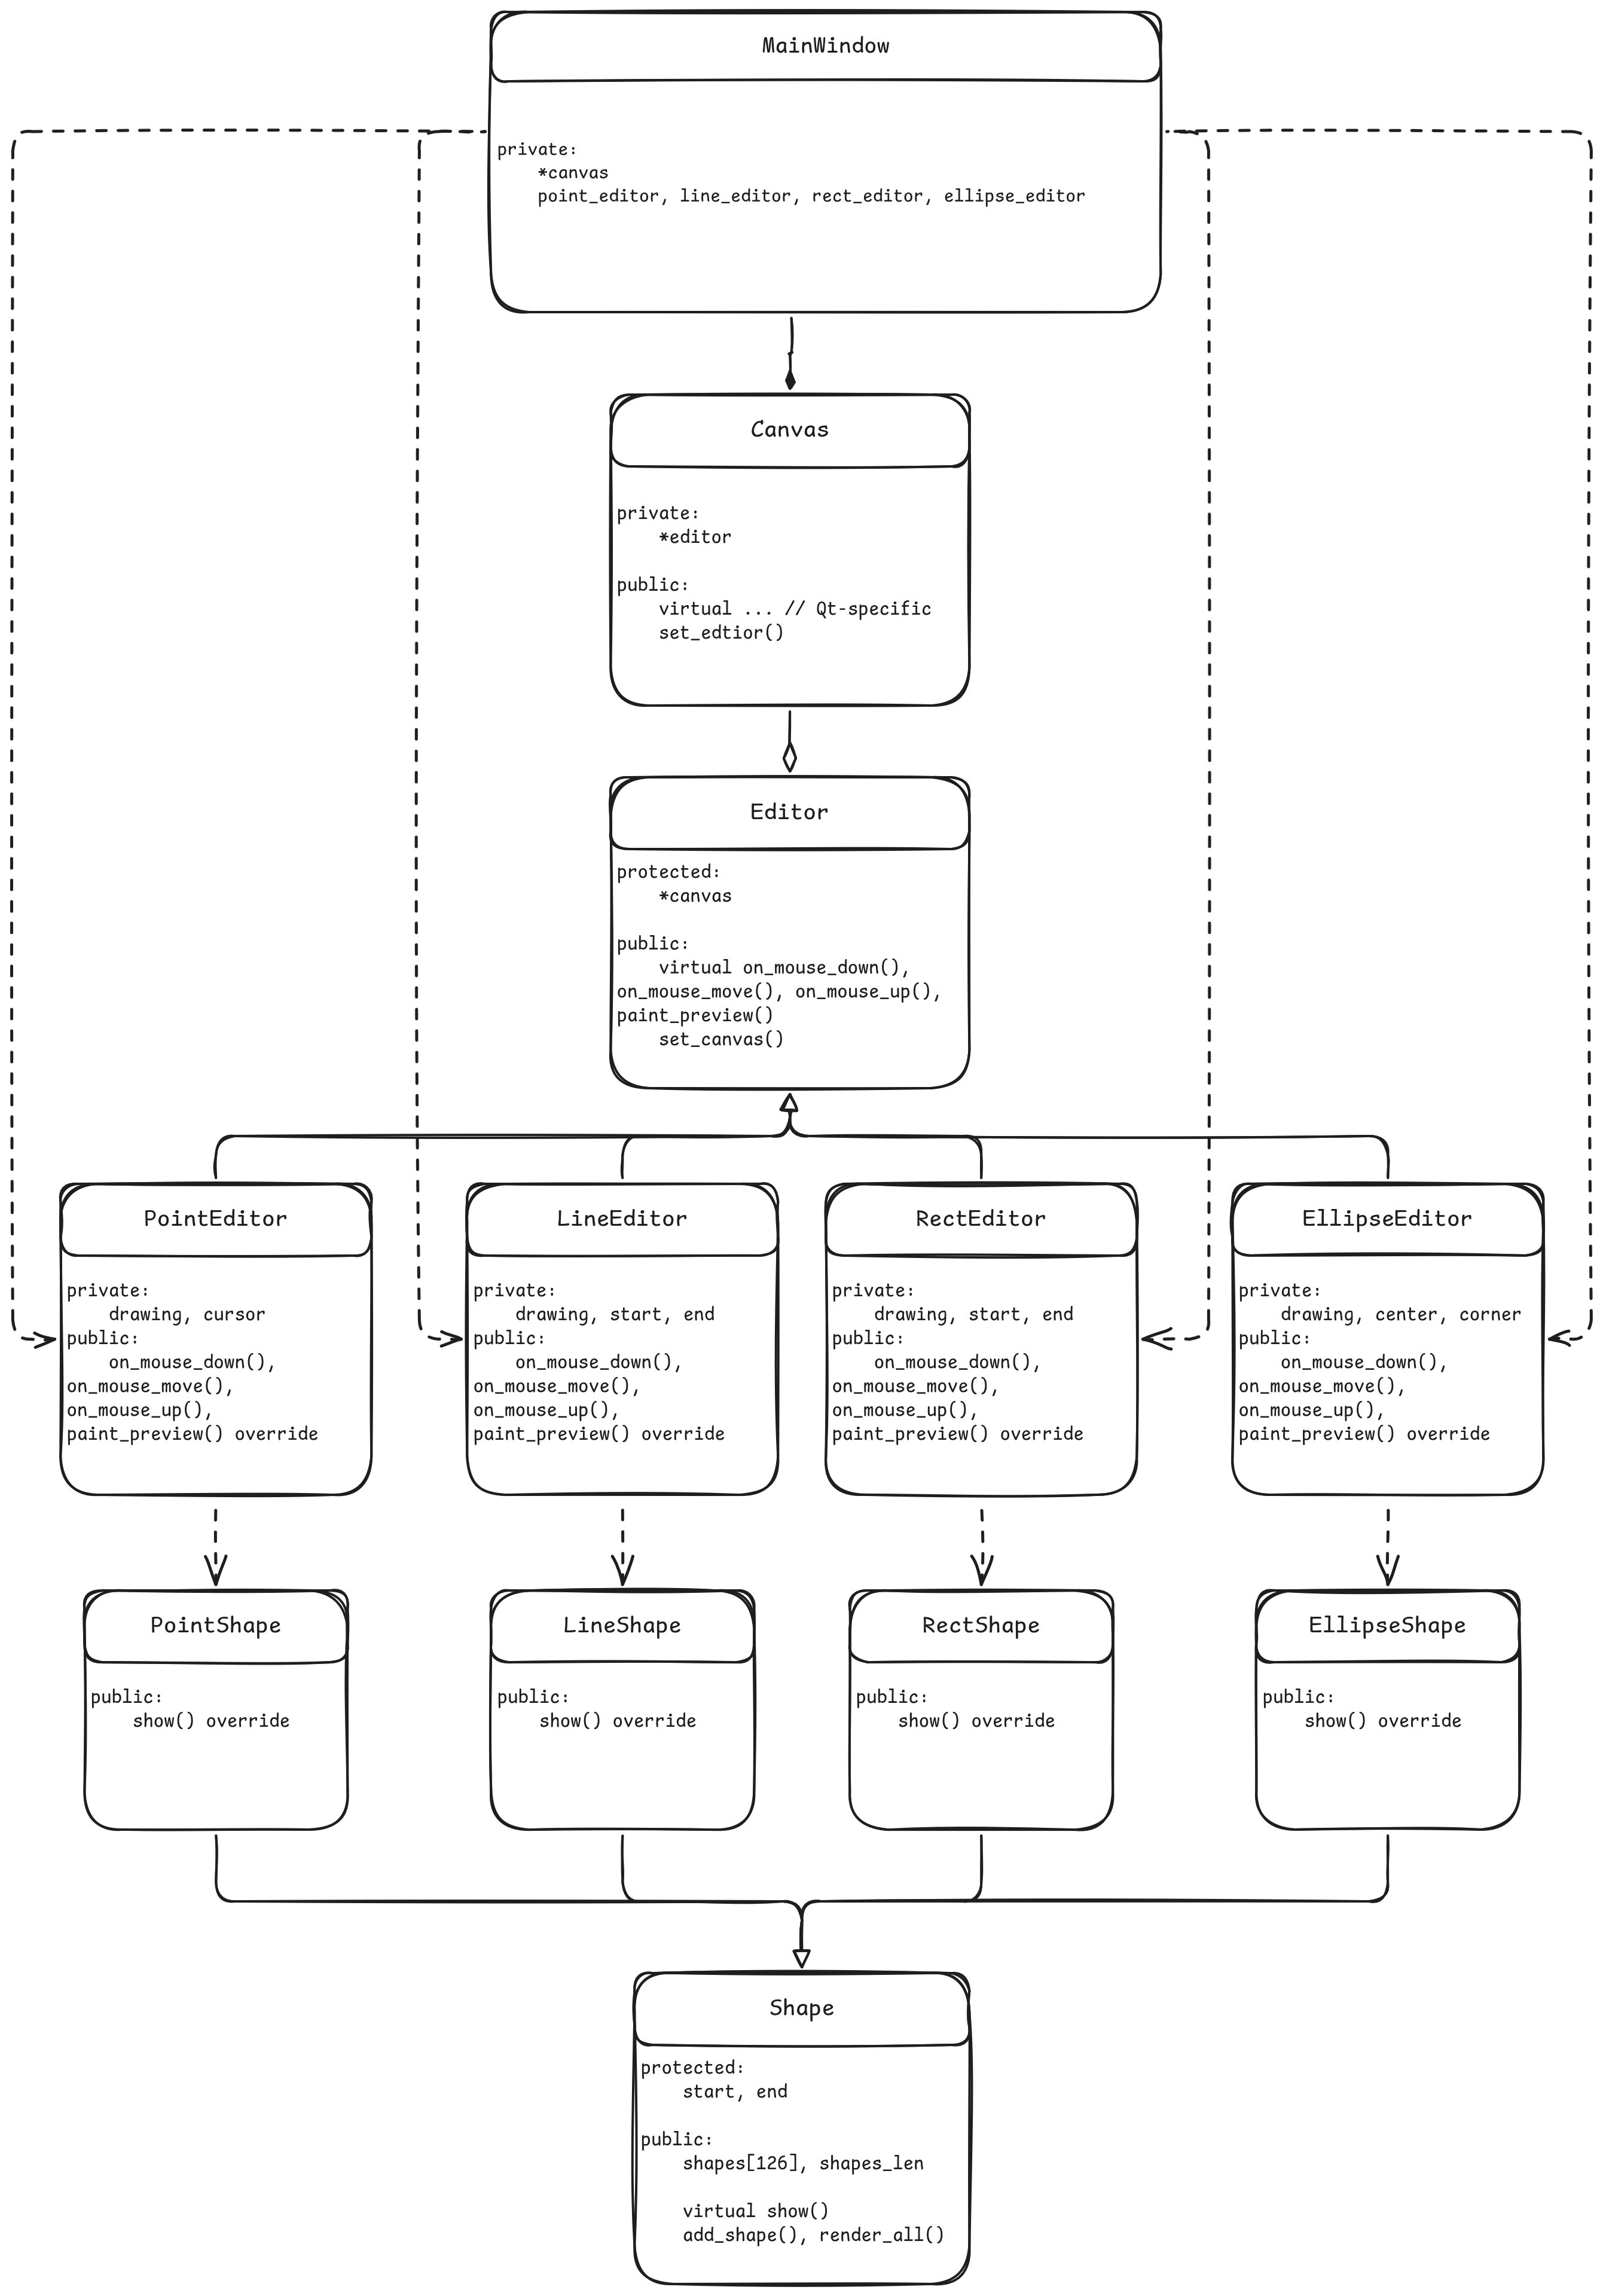
\includegraphics[width=0.8\linewidth]{class_diagram.png}
	\caption{Класова діаграма}
\end{figure}
\begin{figure}[p]
  \center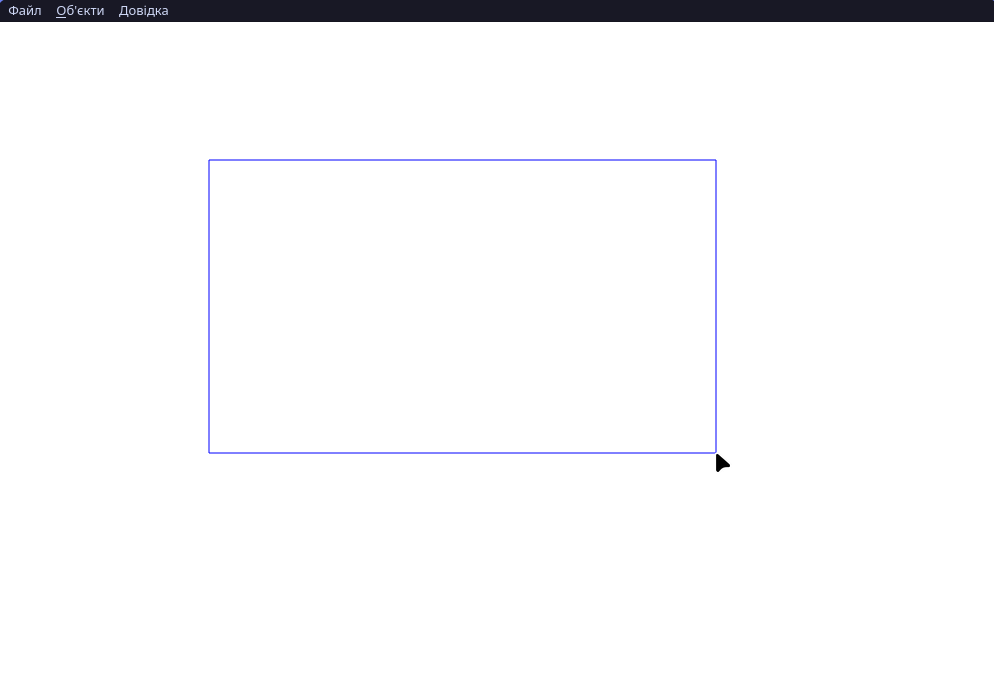
\includegraphics[width=0.7\linewidth]{preview.png}
	\caption{<<Гумовий>> слід}
\end{figure}
\begin{figure}[p]
  \center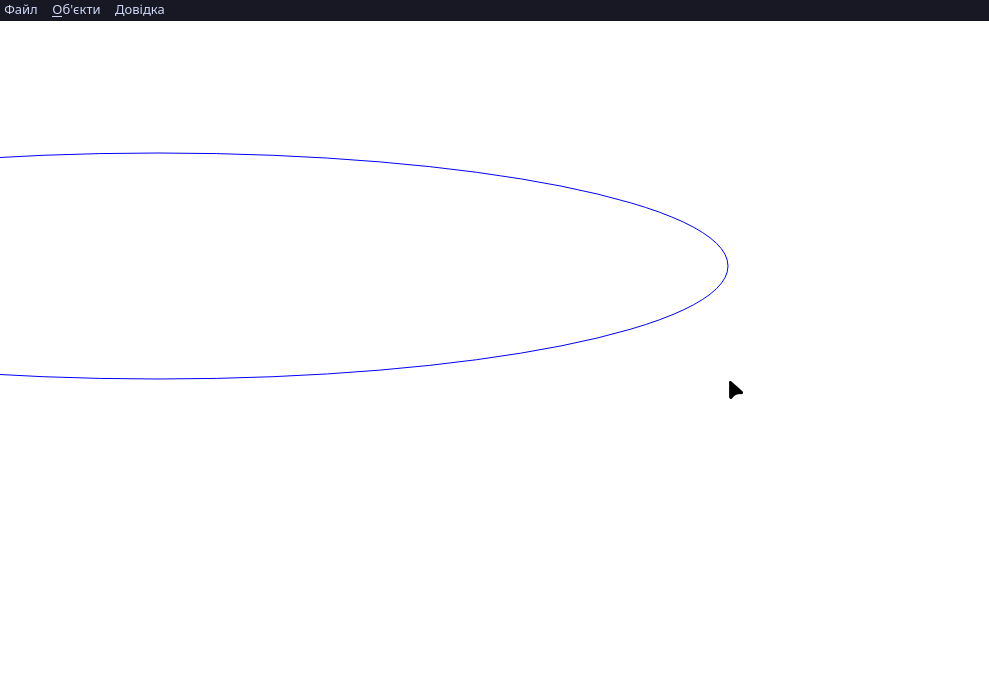
\includegraphics[width=0.7\linewidth]{ellipse.png}
	\caption{Увід еліпса від центра до кута}
\end{figure}
\begin{figure}[t]
  \center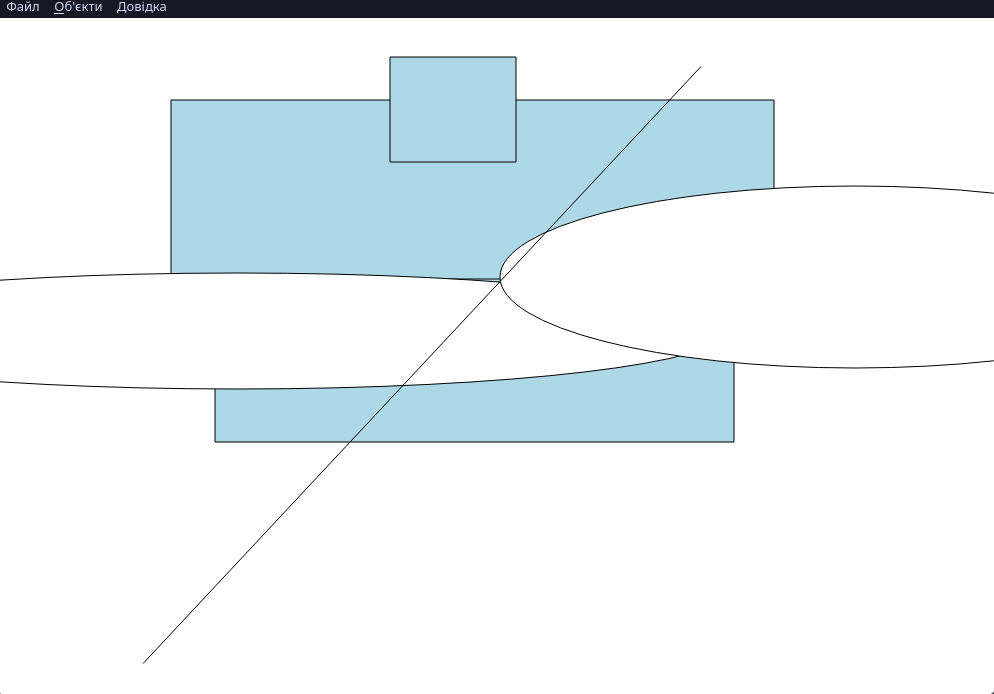
\includegraphics[width=0.7\linewidth]{overlapping.png}
	\caption{Накладання різних фігур}
\end{figure}

\pagebreak

\conclusion%
Реалізував застосунок для малювання геометричних примітивів.
Створив ієрархію класів, де існує кілька конкретних реалізацій для різних
фігур, і відповідний метод відображення викликається поліморфно.
Зобразив діаграму класів.
\end{document}

% vim: ts=2: sw=2
